\let\negmedspace\undefined
\let\negthickspace\undefined
\documentclass[journal]{IEEEtran}
\usepackage[a5paper, margin=10mm, onecolumn]{geometry}
%\usepackage{lmodern} % Ensure lmodern is loaded for pdflatex
\usepackage{tfrupee} % Include tfrupee package

\setlength{\headheight}{1cm} % Set the height of the header box
\setlength{\headsep}{0mm}     % Set the distance between the header box and the top of the text

\usepackage{gvv-book}
\usepackage{gvv}
\usepackage{cite}
\usepackage{amsmath,amssymb,amsfonts,amsthm}
\usepackage{algorithmic}
\usepackage{graphicx}
\usepackage{textcomp}
\usepackage{xcolor}
\usepackage{txfonts}
\usepackage{listings}
\usepackage{enumitem}
\usepackage{mathtools}
\usepackage{gensymb}
\usepackage{tfrupee}
\usepackage[breaklinks=true]{hyperref}
\usepackage{tkz-euclide} 
\usepackage{listings}
% \usepackage{gvv}                                        
\def\inputGnumericTable{}                                 
\usepackage[latin1]{inputenc}                                
\usepackage{color}                                            
\usepackage{array}                                            
\usepackage{longtable}                                       
\usepackage{calc}                                             
\usepackage{multirow}                                         
\usepackage{hhline}                                           
\usepackage{ifthen}                                           
\usepackage{lscape}
\usepackage{circuitikz}
\usepackage{comment}
\tikzstyle{block} = [rectangle, draw, fill=blue!20, 
    text width=4em, text centered, rounded corners, minimum height=3em]
\tikzstyle{sum} = [draw, fill=blue!10, circle, minimum size=1cm, node distance=1.5cm]
\tikzstyle{input} = [coordinate]
\tikzstyle{output} = [coordinate]


\begin{document}

\bibliographystyle{IEEEtran}
\vspace{3cm}
\title{7.4.25}
\author{EE25BTECH11018-Darisy Sreetej}
 \maketitle
% \newpage
% \bigskip
{\let\newpage\relax\maketitle}

\renewcommand{\thefigure}{\theenumi}
\renewcommand{\thetable}{\theenumi}
\setlength{\intextsep}{10pt} % Space between text and floats


\numberwithin{equation}{enumi}
\numberwithin{figure}{enumi}
\renewcommand{\thetable}{\theenumi}

\textbf{Question}:
The locus of the centre of a circle, which touches the circle is $x^2 + y^2 -6x -6y +14 =0$ and also touches the y-axis, is given by the equation:
\begin{enumerate}
    \item $x^2-6x-10y+14=0$
    \item $x^2-10x-6y+14=0$
    \item $y^2-6x-10y+14=0$
    \item $y^2-10x-6y+14=0$
\end{enumerate}
\textbf{Solution}:\\
Given circle equation is ,
$$x^2 + y^2 -6x -6y +14 =0$$
can be represented as 
\begin{align}
    \norm{\vec{x}}^2+2\myvec{-3\\-3}^\top\vec{x}+14=0
\end{align}
The centre of circle is $\vec{c}_1=\myvec{3\\3}$ and radius $r=2$ $\brak{\because f= 14 ,\quad \vec{u}=\myvec{-3\\-3}} $\\
Let the centre of the moving circle be $\vec{c}=\myvec{h\\k}$\\
As the circle touches $X-$axis , Distance of a point from $x$-axis is given by
\begin{align}
    R=|\vec{n}^\top\vec{c}|
\end{align}
where $\vec{n}$ is the unit vector normal to $x$-axis\\
\begin{align}
 \vec{n}=\myvec{1\\0}
\end{align}
Distance between their centers equal to sum of their radius
\begin{align}
    \norm{\vec{c}-\vec{c_1}}&=R \pm r\\
\norm{\vec{c}-\vec{c_1}}&=|\vec{n}^\top\vec{c}| \pm r \\
\norm{\vec{c}-\vec{c_1}}^2&=\brak{|\vec{n}^\top\vec{c}| \pm r}^2 
\end{align}
\begin{align}
\brak{\vec{c}-\vec{c_1}}\brak{\vec{c}-\vec{c_1}}^\top=\brak{|\vec{n}^\top\vec{c}| \pm r}^2 
\end{align}
\begin{align}
\vec{c}^\top\vec{c}+\vec{c_1}\vec{c_1}^\top-\vec{c_1}^\top\vec{c}-\vec{c}^\top\vec{c_1}&= \brak{|\vec{n}^\top\vec{c}|}^2 \pm 2r|\vec{n}^\top\vec{c}|+r^2\\
\vec{c}^\top\vec{c}+\vec{c_1}\vec{c_1}^\top-\vec{c_1}^\top\vec{c}-\vec{c}^\top\vec{c_1}&= \brak{\vec{n}^\top\vec{c}}^\top\brak{\vec{n}^\top\vec{c}}  \pm 2r|\vec{n}^\top\vec{c}|+r^2\\
\vec{c}^\top\vec{c}+\norm{\vec{c_1}}^2-2\vec{c_1}^\top\vec{c}&=\brak{\vec{c}^\top\vec{n}\vec{n}^\top\vec{c}} \pm 2r|\vec{n}^\top\vec{c}|+r^2
\end{align}
\begin{align}
\vec{c}^\top\vec{c}+18&=\brak{\vec{c}^\top\vec{n}\vec{n}^\top\vec{c}}+2\vec{n}^\top\vec{c} \pm 2r|\vec{n}^\top\vec{c}|+ r^2 + 2\vec{c_1}^\top\vec{c}\\
\vec{c}^\top\vec{c}+14&=\brak{\vec{c}^\top\vec{n}\vec{n}^\top\vec{c}}+2\vec{n}^\top\vec{c} \pm 4|\vec{n}^\top\vec{c}| + 2\vec{c_1}^\top\vec{c} \quad (\text{Since r=2})
\end{align}
Case 1 : (External Tangency)
\begin{align}
\vec{c}^\top\vec{c}+14&=\brak{\vec{c}^\top\vec{n}\vec{n}^\top\vec{c}}+2\vec{n}^\top\vec{c} + 4|\vec{n}^\top\vec{c}| + 2\vec{c_1}^\top\vec{c}
\end{align}
\begin{align}
\myvec{x&y}\myvec{x\\y} +14 = \myvec{x&0}\myvec{x\\0} + 4 \brak{\myvec{1 & 0}\myvec{x\\y}} + 2\brak{\myvec{3&3}\myvec{x\\y}}
\end{align}
\begin{align}
x^2+y^2+14=x^2+4x+6x+6y\\
y^2-10x-6y+14=0
\end{align}
Case 2 : (Internal Tangency)
\begin{align}
\vec{c}^\top\vec{c}+14&=\brak{\vec{c}^\top\vec{n}\vec{n}^\top\vec{c}}+2\vec{n}^\top\vec{c} - 4|\vec{n}^\top\vec{c}| + 2\vec{c_1}^\top\vec{c}
\end{align}
\begin{align}
\myvec{x&y}\myvec{x\\y} +14 = \myvec{x&0}\myvec{x\\0} - 4 \brak{\myvec{1 & 0}\myvec{x\\y}} + 2\brak{\myvec{3&3}\myvec{x\\y}}
\end{align}
\begin{align}
x^2+y^2+14=x^2-4x+6x+6y\\
y^2-2x-6y+14=0
\end{align}
Therefore , the locus of the centre of a circle is 
$$
 y^2-10x-6y+14=0   \quad  (\text{from the options})
$$
\begin{figure}[H]
   \centering
   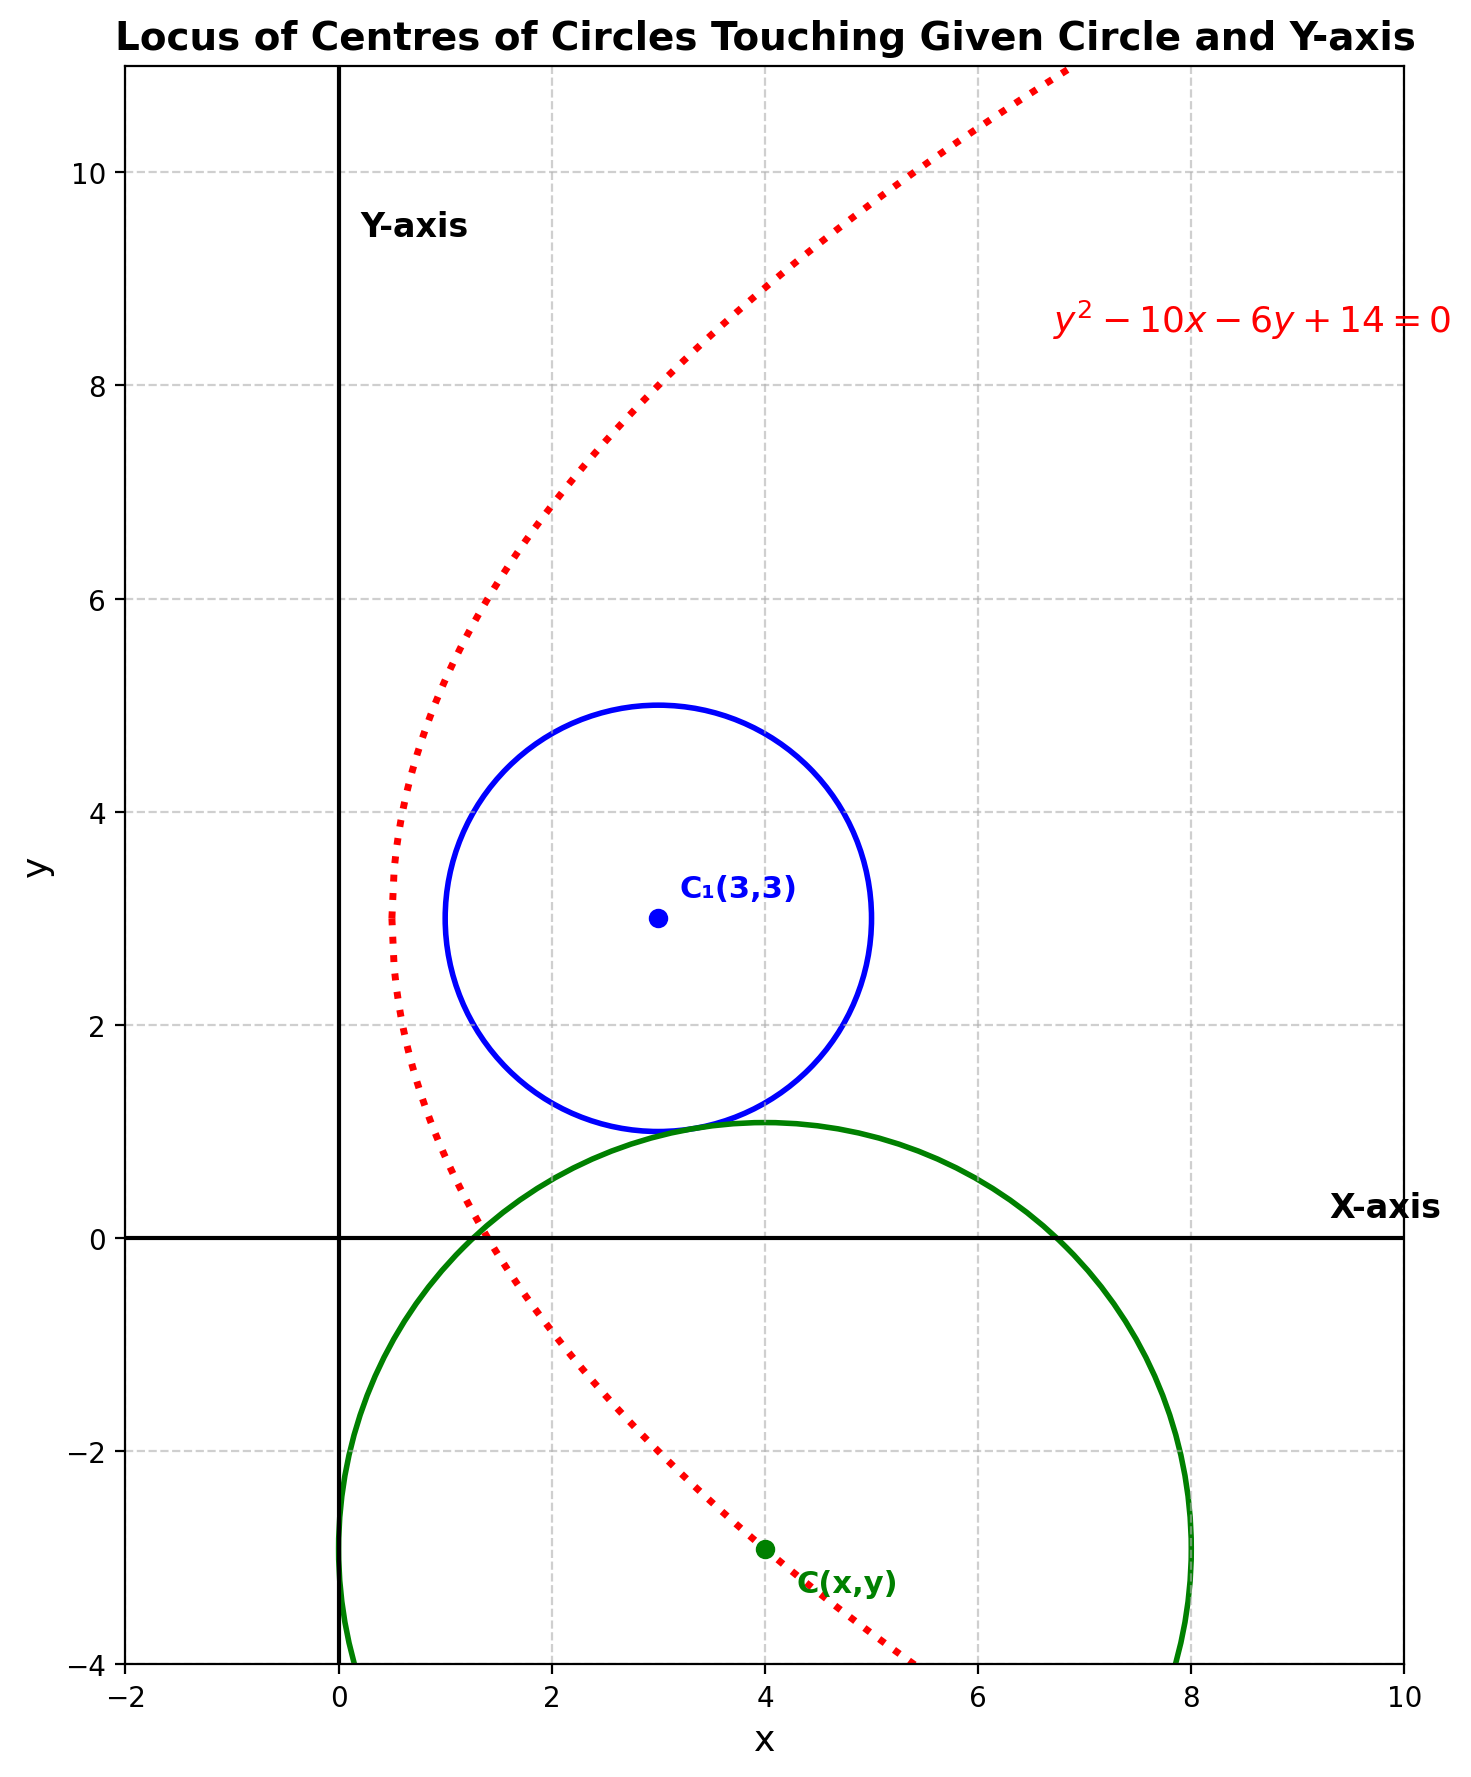
\includegraphics[width=0.7\columnwidth]{figs/fig.png}
	\caption{}
   \label{}
\end{figure}
\end{document}  